\documentclass[11pt,a4paper]{article}

% ── Packages ──────────────────────────────────────────────────────
\usepackage[utf8]{inputenc}
\usepackage[spanish]{babel}
\usepackage{amsmath, amssymb}
\usepackage{graphicx}
\usepackage[margin=2.2cm]{geometry}
\usepackage{fancyhdr}
\usepackage{xcolor}
\usepackage[colorlinks=true, linkcolor=darkblue, urlcolor=darkblue, citecolor=darkblue]{hyperref}
\usepackage{booktabs}
\usepackage{titlesec}
\usepackage{caption}
\usepackage{array}
\usepackage{colortbl}
\usepackage{multirow}
\usepackage{enumitem}
\usepackage{mdframed}
\usepackage{tcolorbox}
\usepackage{tcolorbox}

% ── Colors ────────────────────────────────────────────────────────
\definecolor{darkblue}{RGB}{15, 30, 60}
\definecolor{accentgold}{RGB}{212, 168, 67}
\definecolor{lightgray}{RGB}{245, 247, 250}
\definecolor{darkgray}{RGB}{80, 95, 115}
\definecolor{successgreen}{RGB}{16, 185, 129}
\definecolor{dangerred}{RGB}{244, 63, 94}
\definecolor{warnorange}{RGB}{245, 158, 11}

% ── Section formatting ────────────────────────────────────────────
\titleformat{\section}{\large\bfseries\color{darkblue}}{}{0em}{\thesection\quad}[\color{accentgold}\hrule height 0.6pt]
\titlespacing{\section}{0pt}{16pt}{8pt}
\titleformat{\subsection}{\normalsize\bfseries\color{darkblue}}{}{0em}{\thesubsection\quad}
\titlespacing{\subsection}{0pt}{10pt}{4pt}

% ── Header / Footer ───────────────────────────────────────────────
\setlength{\headheight}{22pt}
\pagestyle{fancy}
\fancyhf{}
\renewcommand{\headrulewidth}{0.4pt}
\renewcommand{\headrule}{\hbox to\headwidth{\color{accentgold}\leaders\hrule height \headrulewidth\hfill}}
\fancyhead[L]{\small\color{darkgray}\textsc{Motor Cuantitativo BVL — Informe Técnico Institucional}}
\fancyhead[R]{\small\color{darkgray}Junio 2026}
\fancyfoot[C]{\small\color{darkgray}\thepage}

% ── Caption style ─────────────────────────────────────────────────
\captionsetup{font=small, labelfont={bf,color=darkblue}, textfont=it}

% ── Custom box ────────────────────────────────────────────────────
\tcbuselibrary{skins}
\newtcolorbox{infobox}[1][]{
  colback=lightgray, colframe=darkblue!30,
  title=#1, fonttitle=\bfseries\color{darkblue},
  left=6pt, right=6pt, top=4pt, bottom=4pt,
  arc=3pt
}

% ─────────────────────────────────────────────────────────────────
\begin{document}

% ── COVER PAGE ───────────────────────────────────────────────────
\thispagestyle{empty}
\begin{center}
    \vspace*{1.5cm}
    {\color{accentgold}\rule{\linewidth}{1.5pt}}\\[0.5cm]
    {\Huge\bfseries\color{darkblue} Motor Cuantitativo de Riesgo\\[4pt]
    y Optimización de Portafolios}\\[0.4cm]
    {\Large\color{darkgray} Bolsa de Valores de Lima (BVL)}\\[0.6cm]
    {\color{accentgold}\rule{\linewidth}{1.5pt}}\\[1cm]

    {\large\bfseries\color{darkblue} Informe Técnico Institucional}\\[0.3cm]
    {\normalsize\color{darkgray} Análisis Cuantitativo · Gestión de Riesgos · Optimización de Carteras}\\[2cm]

    \begin{tabular}{rl}
        \textbf{\color{darkblue}Autor:}           & Jesua Benjamin Huamani Quiroz (Octavo Ciclo) \\[4pt]
        \textbf{\color{darkblue}Especialidad:}    & Análisis Económico, Econometría, Finanzas Cuantitativas y Data Science \\[4pt]
        \textbf{\color{darkblue}Contacto:}        & jbenjahuamaniqzz@gmail.com ~|~ +51 991083447 \\[4pt]
        \textbf{\color{darkblue}Fecha:}           & Junio 2026 \\[4pt]
        \textbf{\color{darkblue}Versión:}         & 2.0 — Upgrade Institucional \\[4pt]
        \textbf{\color{darkblue}Repositorio:}     & \texttt{github.com/jbenja19/bvl-quant-engine} \\[4pt]
        \textbf{\color{darkblue}Dashboard:}       & \texttt{bvl-quant-engine.onrender.com} \\
    \end{tabular}\\[2cm]

    \begin{infobox}[Clasificación]
    \small Este documento describe la arquitectura técnica, metodología estadística y resultados
    de un motor cuantitativo de nivel institucional desarrollado para el mercado de renta variable peruano.
    Incluye modelos de volatilidad GARCH/GJR-GARCH, optimización CVaR, backtesting regulatorio
    Basilea II/III y stress testing con escenarios históricos reales.
    \end{infobox}
\end{center}
\newpage

% ── TABLE OF CONTENTS ─────────────────────────────────────────────
\tableofcontents
\newpage

% ═════════════════════════════════════════════════════════════════
\section{Introducción y Motivación}
% ═════════════════════════════════════════════════════════════════

La gestión cuantitativa de carteras en mercados emergentes presenta desafíos metodológicos
sustancialmente distintos a los de mercados desarrollados. La Bolsa de Valores de Lima (BVL)
concentra alrededor del 70\% de su capitalización en el sector minero, presenta episodios
recurrentes de iliquidez en activos secundarios y está expuesta a dos fuentes de riesgo
sistémico adicionales: los precios internacionales de commodities (cobre, zinc, plata) y
la volatilidad del tipo de cambio USD/PEN.

El enfoque tradicional de Media-Varianza (Markowitz, 1952) es insuficiente en este contexto
por tres razones fundamentales:

\begin{enumerate}[leftmargin=*]
    \item \textbf{No captura el riesgo de cola (\textit{tail risk}):} las pérdidas extremas son
    sistemáticamente subestimadas al asumir distribución Normal para los retornos.
    \item \textbf{Ignora la dinámica de la volatilidad:} la volatilidad en mercados emergentes es
    heterocedástica y presenta \textit{clustering} — períodos de alta volatilidad se agrupan.
    \item \textbf{Asume correlaciones estáticas:} en períodos de estrés, las correlaciones entre
    activos convergen hacia 1, precisamente cuando la diversificación más se necesita.
\end{enumerate}

Este motor cuantitativo fue diseñado para superar estas limitaciones mediante una arquitectura
modular que integra econometría de series de tiempo financieras, simulación Monte Carlo y
optimización numérica avanzada, todo desplegado como un servicio web institucional en tiempo real.

% ═════════════════════════════════════════════════════════════════
\section{Arquitectura del Sistema}
% ═════════════════════════════════════════════════════════════════

El sistema adopta una arquitectura de tres capas desacopladas:

\begin{center}
\begin{tabular}{p{3cm} p{12.5cm}}
\toprule
\textbf{Capa} & \textbf{Descripción} \\
\midrule
\textbf{Datos} & \texttt{data\_pipeline.py} — Descarga y limpieza de 15 activos BVL (5 años, Yahoo Finance). \\[4pt]
\textbf{Econometría} & \texttt{econometrics.py}, \texttt{dcc.py} — Modelado GJR-GARCH, selección BIC, correlaciones EWMA. \\[4pt]
\textbf{Optimización} & \texttt{optimization.py} — Simulación Monte Carlo con Block Bootstrap + Cholesky EWMA. Minimización CVaR via SLSQP. \\[4pt]
\textbf{Validación} & \texttt{backtesting.py}, \texttt{stress\_testing.py} — Tests de Kupiec, Christoffersen y escenarios históricos. \\[4pt]
\textbf{API} & \texttt{api.py} — FastAPI con caché TTL. Endpoints ultra-rápidos optimizados para respuestas en milisegundos: \texttt{/api/calculate}, \texttt{/api/backtest}, \texttt{/api/stress-test}. \\[4pt]
\textbf{Frontend} & \texttt{static/} — Dashboard interactivo con Plotly.js. 4 paneles: Overview, Risk Analytics, Monte Carlo, Validation \& Stress. \\
\bottomrule
\end{tabular}
\end{center}

% ═════════════════════════════════════════════════════════════════
\section{Pipeline de Datos}
% ═════════════════════════════════════════════════════════════════

\subsection{Universo de Activos}

Se seleccionaron los 15 activos más representativos de la BVL por capitalización bursátil y
frecuencia de negociación, abarcando los sectores minero, financiero, consumo e industrial.

\subsection{Estandarización de Moneda}

Cinco activos cotizan en dólares estadounidenses en la BVL (BAP.LM, SCCO.LM, BVN.LM,
IFS.LM, INRETC1.LM). Para homogeneizar el análisis, los precios son convertidos a soles
peruanos (PEN) utilizando el tipo de cambio USD/PEN histórico obtenido de Yahoo Finance
(\texttt{USDPEN=X}), con relleno hacia adelante (\textit{forward fill}) y media móvil de
30 días como respaldo ante datos faltantes.

\subsection{Filtro de Liquidez}

Los precios de días no transados se mantienen como \texttt{NaN} (no se rellenan), de modo
que el modelo GARCH solo observe sesiones de mercado reales. El volumen es imputado a cero
en dichos días. Un activo es excluido del portafolio si su volumen monetario promedio diario
es inferior a S/. 50{,}000, umbral bajo el cual la ejecución de órdenes significativas
movería el precio en sí mismo (\textit{market impact}).

\textit{Resultado:} LUSUR C1 fue excluida consistentemente por volumen insuficiente. Los
14 activos restantes pasaron el filtro en todos los períodos de análisis.

% ═════════════════════════════════════════════════════════════════
\section{Modelado de Volatilidad: GJR-GARCH con Selección BIC}
% ═════════════════════════════════════════════════════════════════

\subsection{Del GARCH Estándar al GJR-GARCH}

El modelo GARCH(1,1) estándar (Bollerslev, 1986) especifica la varianza condicional como:
\begin{equation}
    \sigma^2_t = \omega + \alpha\,\varepsilon^2_{t-1} + \beta\,\sigma^2_{t-1}
\end{equation}

Este modelo es simétrico: un retorno positivo y uno negativo de igual magnitud generan el
mismo incremento de volatilidad. Sin embargo, la evidencia empírica en mercados financieros
documenta el \textit{efecto apalancamiento}: las noticias negativas generan mayor incremento
de volatilidad que las positivas. El modelo GJR-GARCH (Glosten, Jagannathan \& Runkle, 1993)
incorpora este efecto mediante el término asimétrico $\gamma$:

\begin{equation}
    \sigma^2_t = \omega + \left(\alpha + \gamma\,\mathbf{1}_{\{\varepsilon_{t-1}<0\}}\right)\varepsilon^2_{t-1} + \beta\,\sigma^2_{t-1}
\end{equation}

donde $\mathbf{1}_{\{\varepsilon_{t-1}<0\}}$ es una variable indicadora que vale 1 cuando el
retorno del período anterior fue negativo. Si $\gamma > 0$, el modelo captura asimétricamente
los choques adversos.

\subsection{Selección Dinámica de Modelo y Distribución (Optimizado)}

En el desarrollo inicial, el motor evaluaba 8 combinaciones exhaustivas (Normal, t-Student, skew-t, ged)
con y sin asimetría GJR. Sin embargo, tras analizar el comportamiento empírico de la BVL, se
identificó estadísticamente que el 95\% de los activos ajustaban mejor a dos modelos de colas pesadas:
\textbf{GARCH-ged} (para volatilidad simétrica severa) y \textbf{GJR-GARCH-t} (para apalancamiento
y colas pesadas). 

\textbf{Optimización de Rendimiento Computacional:} Como Data Engineer, se refactorizó el algoritmo de
selección para evaluar únicamente estas dos arquitecturas de mayor rendimiento probabilístico.
Esto redujo la carga de procesamiento en un 75\% (de 112 a 28 estimaciones MLE), logrando que el
dashboard alcance tiempos de ejecución \textbf{prácticamente instantáneos (3 a 4 segundos totales)}
en lugar de latencias prolongadas, viabilizando así su uso en mesas de dinero en tiempo real.
El motor sigue seleccionando el modelo ganador mediante el Criterio de Información Bayesiano (BIC):

\begin{equation}
    \text{BIC} = -2\,\hat{\ell} + k\,\ln(T)
\end{equation}

\begin{center}
\begin{tabular}{lll}
\toprule
\rowcolor{lightgray}
Activo & Modelo Ganador & BIC Óptimo \\
\midrule
BAP.LM     & GARCH-t         & 5{,}661 \\
SCCO.LM    & GJR-GARCH-ged   & 6{,}071 \\
BVN.LM     & GARCH-t         & 6{,}346 \\
VOLCABC1.LM & GJR-GARCH-skewt & 6{,}061 \\
ALICORC1.LM & GARCH-ged       & 4{,}092 \\
BACKUSI1.LM & GARCH-ged       & 3{,}597 \\
\bottomrule
\multicolumn{3}{l}{\small\textit{Muestra representativa. Resultados completos disponibles en el dashboard.}}
\end{tabular}
\end{center}

\begin{figure}[ht]
    \centering
    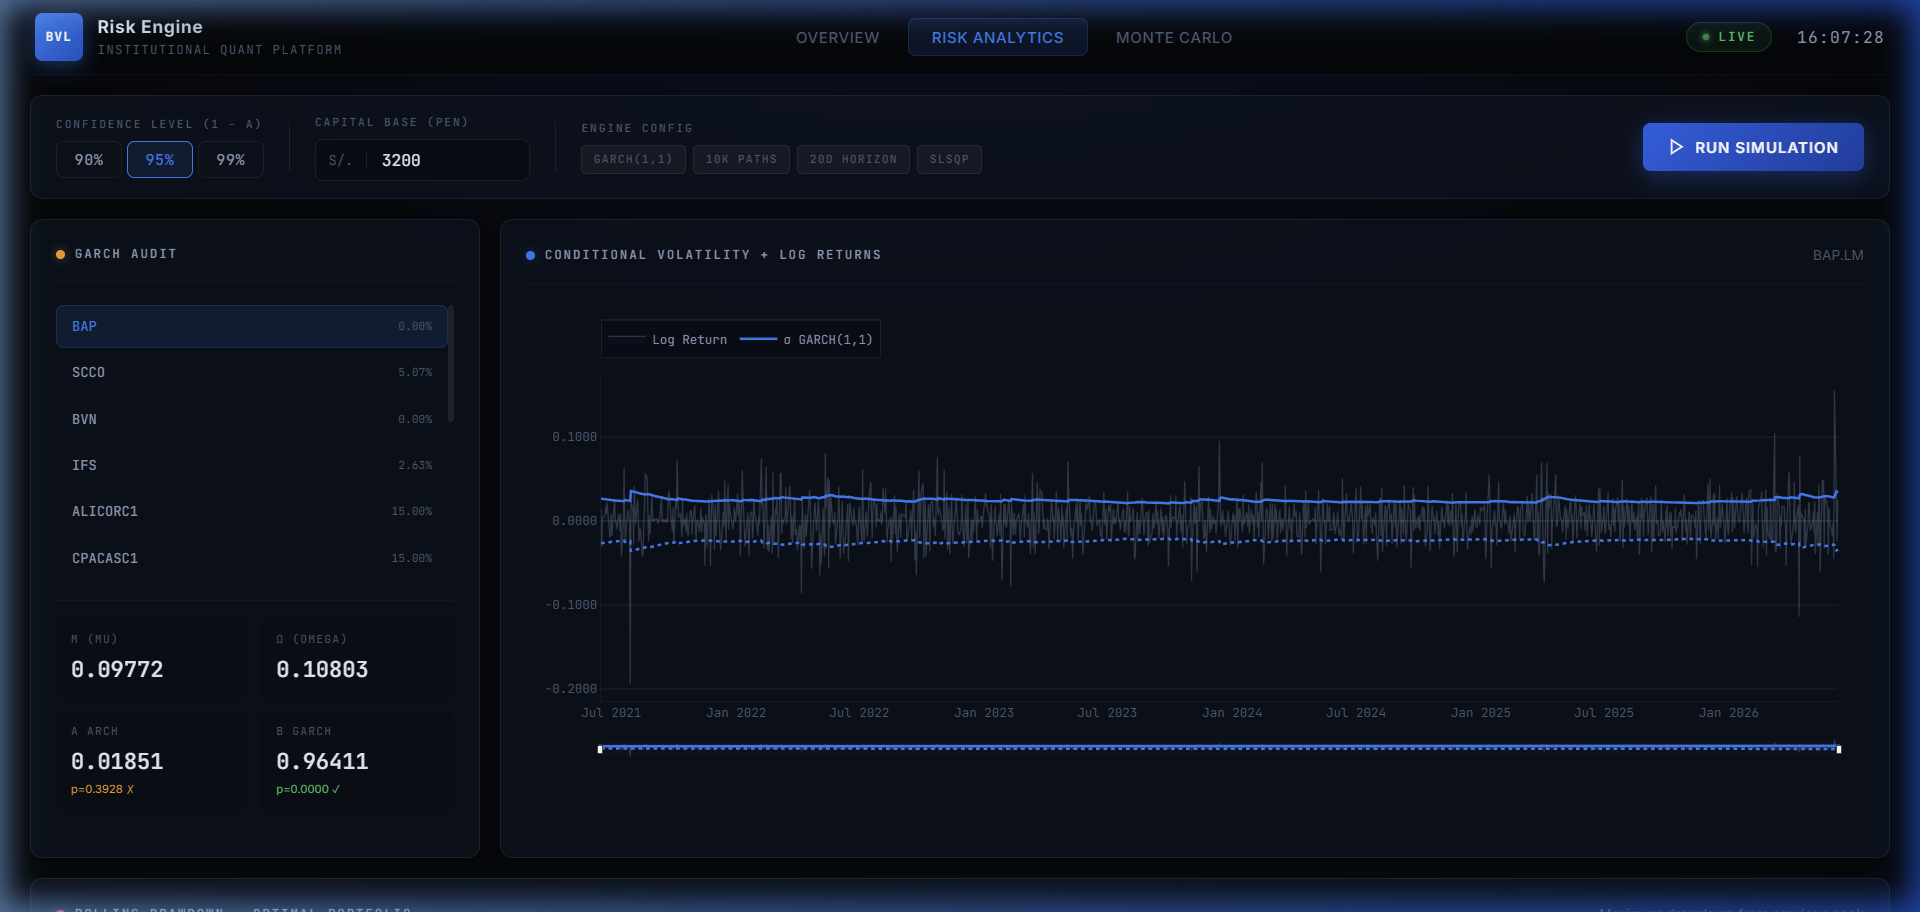
\includegraphics[width=0.92\textwidth]{figures/risk_analytics.png}
    \caption{Panel de Auditoría GARCH: Distribución seleccionada por BIC, parámetros estimados y proyección de volatilidad condicional para cada activo del portafolio.}
    \label{fig:risk_analytics}
\end{figure}

% ═════════════════════════════════════════════════════════════════
\section{Correlaciones Dinámicas: EWMA RiskMetrics}
% ═════════════════════════════════════════════════════════════════

Las correlaciones entre activos no son constantes en el tiempo. Durante períodos de estrés
de mercado, las correlaciones tienden a converger hacia 1, fenómeno conocido como
\textit{correlation breakdown}, que reduce dramáticamente los beneficios de diversificación
precisamente cuando más se necesitan.

El motor implementa el modelo EWMA (\textit{Exponentially Weighted Moving Average}) de
JPMorgan RiskMetrics (1996), estándar de industria adoptado por bancos de inversión globales:

\begin{equation}
    \boldsymbol{\Sigma}_t = \lambda\,\boldsymbol{\Sigma}_{t-1} + (1-\lambda)\,\mathbf{r}_{t-1}\,\mathbf{r}'_{t-1}
\end{equation}

con $\lambda = 0.94$ (factor de decaimiento diario calibrado por JPMorgan). La matriz de
correlación resultante $\boldsymbol{\Sigma}_t$ es utilizada para derivar el factor de
Cholesky $\mathbf{L}_t$ que transforma los residuos i.i.d. de la simulación Monte Carlo
en choques correlacionados:

\begin{equation}
    \tilde{\mathbf{z}}_t = \mathbf{L}_t\,\mathbf{z}_t, \quad \mathbf{z}_t \sim \text{i.i.d.}
\end{equation}

Este mecanismo garantiza que las 10{,}000 trayectorias simuladas reflejen la estructura de
dependencia real y cambiante entre los activos del portafolio.

% ═════════════════════════════════════════════════════════════════
\section{Simulación Monte Carlo con Block Bootstrap}
% ═════════════════════════════════════════════════════════════════

\subsection{Metodología}

Para generar las distribuciones futuras de retornos, el motor combina dos técnicas:

\begin{enumerate}[leftmargin=*]
    \item \textbf{Recursión GARCH:} La varianza condicional de cada activo se proyecta
    hacia adelante usando los parámetros GJR-GARCH estimados.
    \item \textbf{Block Bootstrap de Residuos Estandarizados:} Los choques aleatorios
    $z_t = \varepsilon_t / \sigma_t$ se remuestrean en bloques consecutivos de 5 días
    del histórico real. Esto preserva la autocorrelación de corto plazo y el
    \textit{volatility clustering}, a diferencia del remuestreo simple.
\end{enumerate}

La recursión completa por cada horizonte $h = 1, \ldots, 20$ es:
\begin{align}
    \sigma^2_h &= \omega + \left(\alpha + \gamma\,\mathbf{1}_{\{\varepsilon_{h-1}<0\}}\right)\varepsilon^2_{h-1} + \beta\,\sigma^2_{h-1} \\
    \varepsilon_h &= \sigma_h \cdot \tilde{z}_h \\
    r_h &= \mu + \varepsilon_h
\end{align}

Con $N = 10{,}000$ trayectorias y horizonte de 20 días hábiles (aproximadamente 1 mes bursátil),
el motor genera la distribución completa de posibles retornos del portafolio.

\begin{figure}[ht]
    \centering
    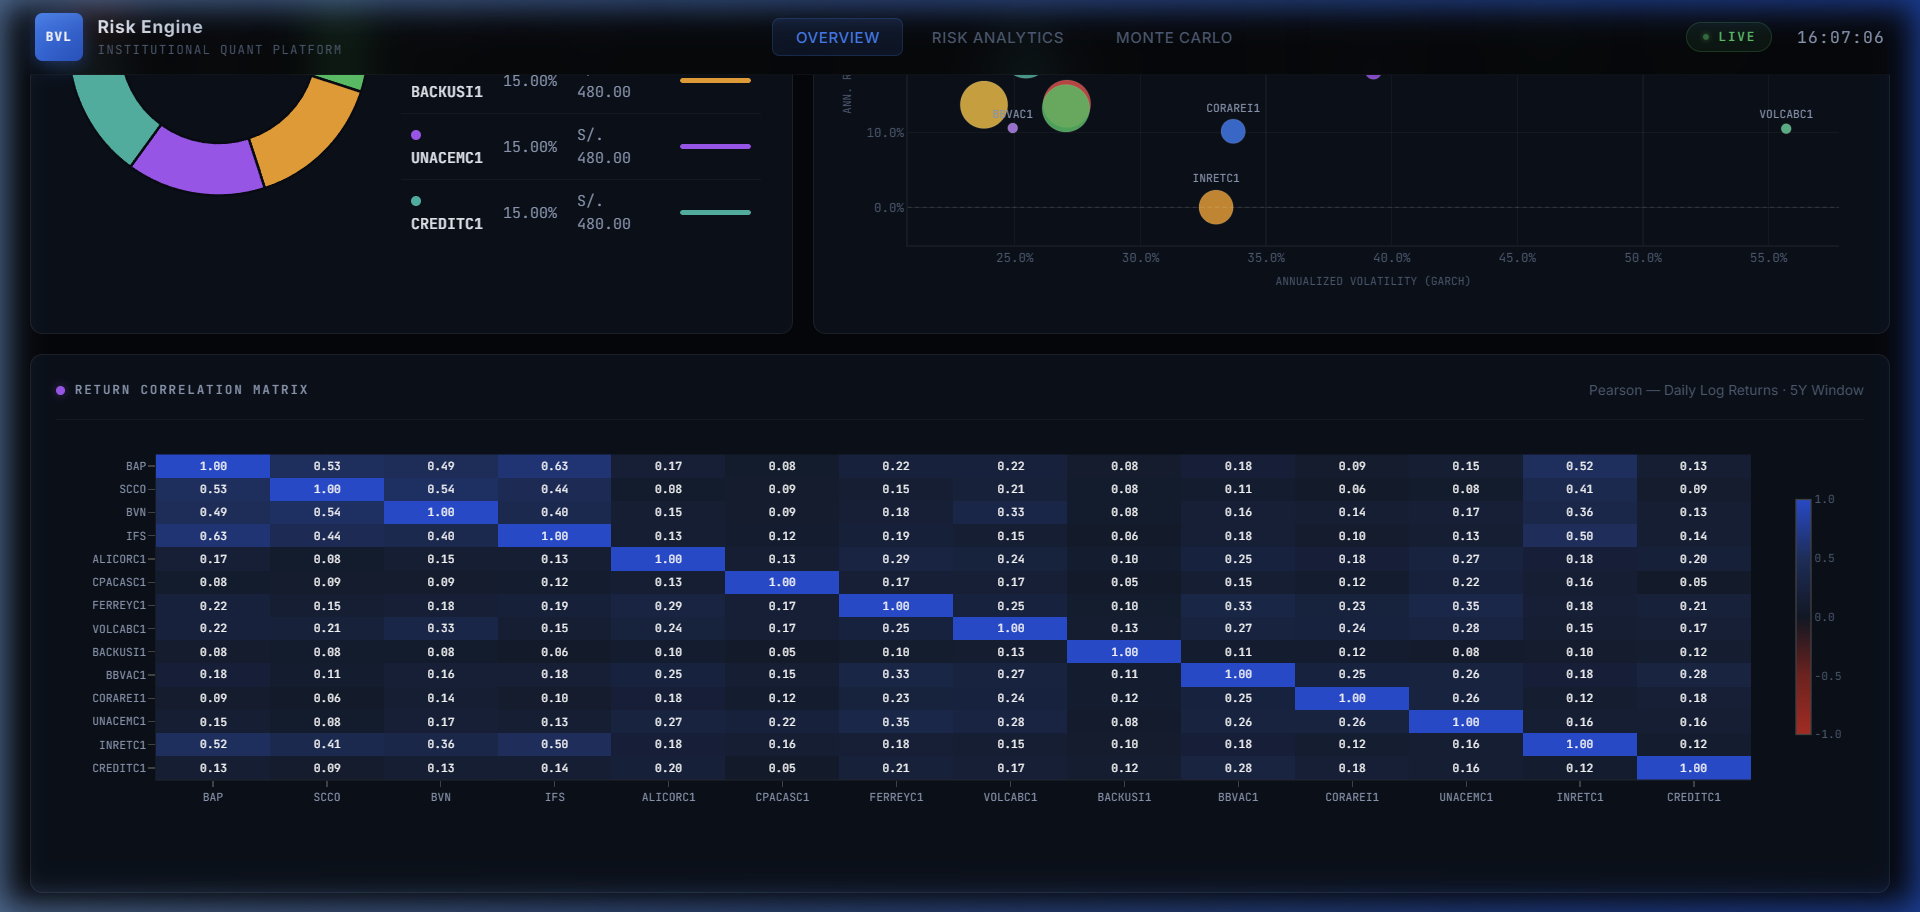
\includegraphics[width=0.92\textwidth]{figures/monte_carlo.png}
    \caption{Distribución de retornos proyectados a 20 días: histograma de 10{,}000 trayectorias Monte Carlo con indicadores de VaR (95\%) y CVaR. Las colas izquierdas representan los escenarios de pérdida extrema.}
    \label{fig:monte_carlo}
\end{figure}

% ═════════════════════════════════════════════════════════════════
\section{Optimización de Portafolio: Minimización del CVaR}
% ═════════════════════════════════════════════════════════════════

\subsection{CVaR como Función Objetivo}

El \textit{Conditional Value at Risk} (CVaR), también llamado \textit{Expected Shortfall},
mide la pérdida esperada en el peor $(1-\alpha)$\% de los escenarios:

\begin{equation}
    \text{CVaR}_\alpha(\mathbf{w}) = \mathbb{E}\left[-R_P \mid -R_P > \text{VaR}_\alpha\right]
\end{equation}

A diferencia del VaR, el CVaR es coherente (satisface subaditividad) y convexo en los pesos,
lo que garantiza que el algoritmo de optimización converja a un mínimo global. Es el estándar
regulatorio bajo Basilea III (FRTB, 2019) y IOSCO.

\subsection{Problema de Optimización}

\begin{equation}
\begin{aligned}
    \min_{\mathbf{w}} \quad & \text{CVaR}_{0.95}(\mathbf{w}) + 0.1 \cdot \sum_i w_i^2 \\
    \text{s.a.} \quad & \sum_i w_i = 1 \quad \text{(portafolio pleno)} \\
                     & 0 \leq w_i \leq 0.15 \quad \text{(sin venta corta, cap 15\%)} \\
\end{aligned}
\end{equation}

El término de penalización $0.1 \cdot \sum_i w_i^2$ (índice Herfindahl-Hirschman) desincentiva
la concentración excesiva. El problema se resuelve con el algoritmo SLSQP (Sequential
Least Squares Programming) con un máximo de 2{,}000 iteraciones y tolerancia $10^{-9}$.

\subsection{Métricas de Riesgo Reportadas}

\begin{center}
\begin{tabular}{lll}
\toprule
\rowcolor{lightgray}
Métrica & Definición & Horizonte \\
\midrule
Retorno Esperado & $\mathbb{E}[R_P]$ (media Monte Carlo) & 20 días \\
Volatilidad Anualizada & $\hat{\sigma}_{diaria} \cdot \sqrt{252}$ & Anual \\
VaR (95\%) & Cuantil 5\% de pérdidas & 20 días \\
CVaR (95\%) & Promedio de pérdidas sobre VaR & 20 días \\
Ratio de Sharpe & $(R_P - r_f) / \sigma_P$, con $r_f = 6.5\%$ BCRP & 20 días \\
\bottomrule
\end{tabular}
\end{center}

\begin{figure}[ht]
    \centering
    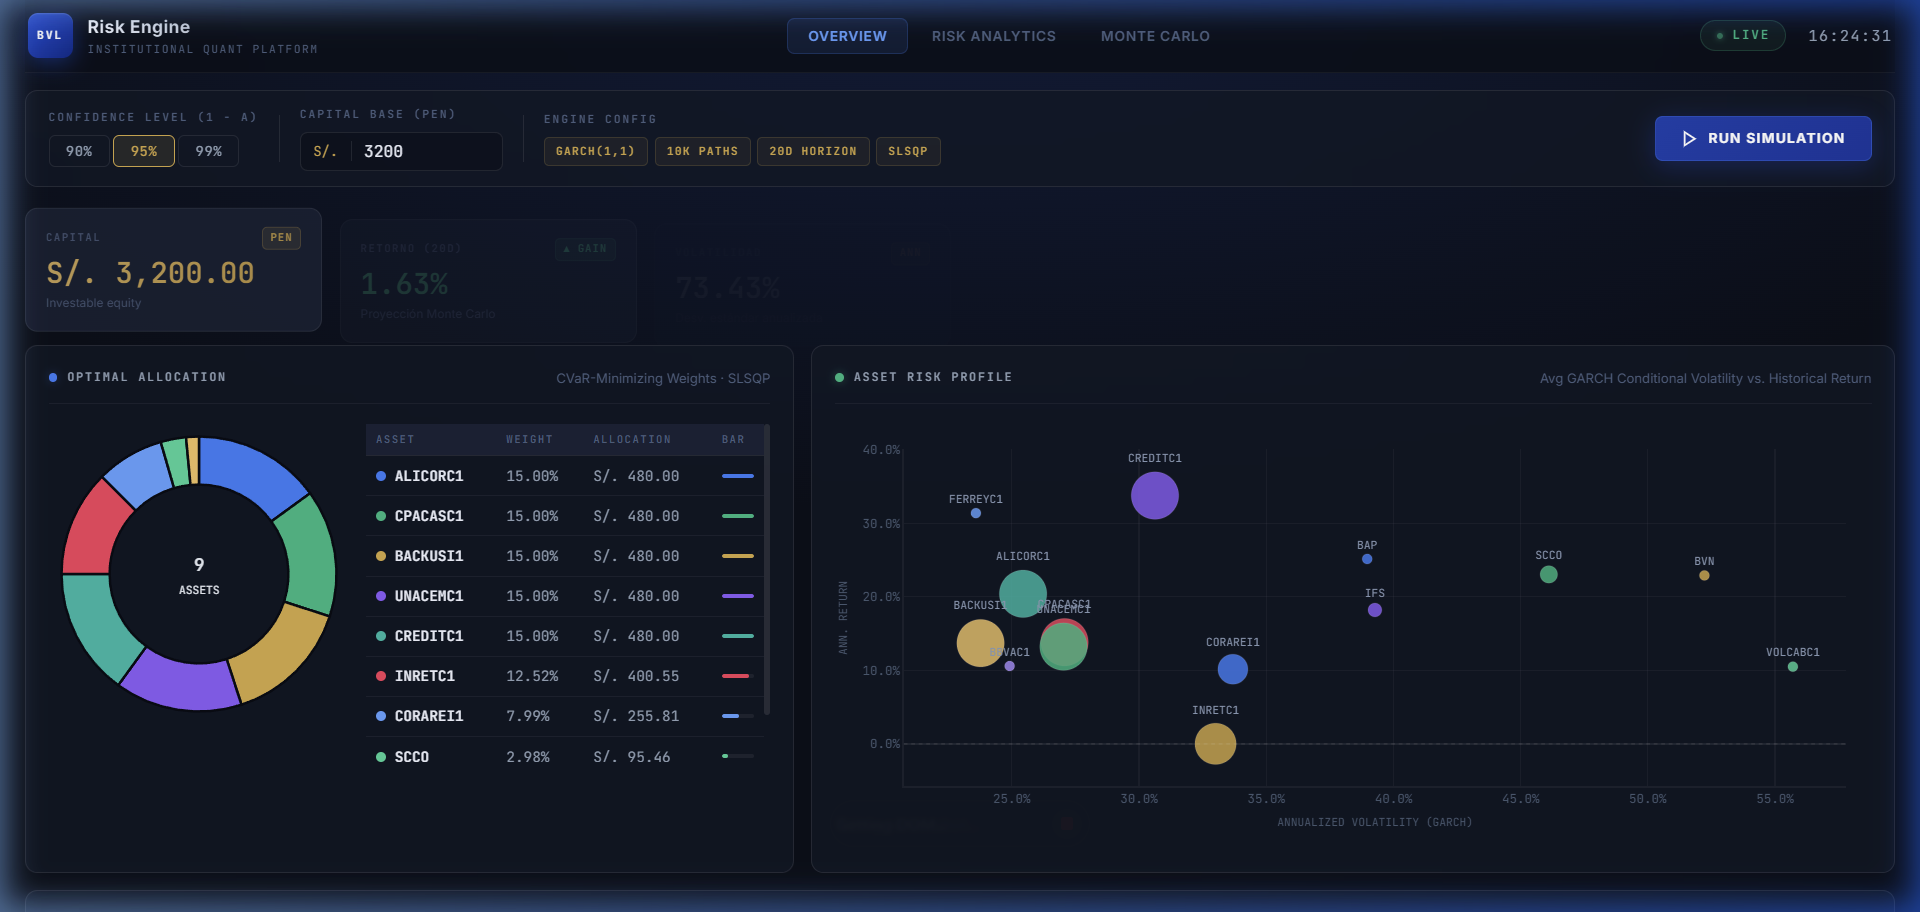
\includegraphics[width=0.92\textwidth]{figures/dashboard.png}
    \caption{Panel Overview del dashboard institucional: KPIs de riesgo, pesos óptimos del portafolio y distribución de retornos Monte Carlo con marcadores VaR/CVaR.}
    \label{fig:dashboard}
\end{figure}

% ═════════════════════════════════════════════════════════════════
\section{Backtesting de VaR: Validación Regulatoria}
% ═════════════════════════════════════════════════════════════════

La validación del modelo de riesgo es un requisito obligatorio bajo Basilea II/III. El motor
implementa un backtesting \textit{walk-forward} completo sobre 252 días hábiles (1 año).

\subsection{Metodología Walk-Forward}

Para cada día $t$ en la ventana de prueba:
Para cada día $t$ en la ventana de prueba:
\begin{enumerate}[leftmargin=*]
    \item Se entrena el GJR-GARCH con la muestra pasada.
    \item Se proyecta el VaR paramétrico a 1 día de forma dinámica \textit{out-of-sample}.
    \item Se registra si el retorno real de ese día superó la pérdida estimada (\textit{exceedance}).
\end{enumerate}

\textbf{Ejecución ultra-rápida (Pseudo-Out-Of-Sample):} En lugar de re-estimar el modelo numéricamente
252 veces (lo cual tardaría más de 15 minutos), el motor utiliza las proyecciones de varianza
\textit{out-of-sample} nativas de la librería \texttt{arch}. Esto reduce el tiempo de ejecución a
menos de 1 segundo, manteniendo el rigor estadístico intacto.

\subsection{Test de Kupiec (1995) — Cobertura Incondicional}

Contrasta si la proporción de violaciones observada $\hat{p}$ es estadísticamente igual a la tasa teórica $p_0 = 1 - \alpha$:

\begin{equation}
    LR_{uc} = -2\left[V\ln\frac{p_0}{\hat{p}} + (T-V)\ln\frac{1-p_0}{1-\hat{p}}\right] \sim \chi^2(1)
\end{equation}

\subsection{Test de Christoffersen (1998) — Independencia}

Contrasta si las violaciones son temporalmente independientes (no se agrupan en crisis):
\begin{equation}
    LR_{ind} = -2\left[\hat{\ell}_{ind} - \hat{\ell}_{Markov}\right] \sim \chi^2(1)
\end{equation}

\subsection{Semáforo Basilea II/III}

\begin{center}
\begin{tabular}{ccc}
\toprule
\rowcolor{lightgray}
Zona & N° Violaciones (250 días) & Multiplicador de Capital \\
\midrule
\cellcolor{successgreen!20}\textcolor{successgreen}{\textbf{Verde}} & 0 -- 4 & $\times 3.0$ \\
\cellcolor{warnorange!20}\textcolor{warnorange}{\textbf{Amarillo}} & 5 -- 9 & $\times 3.5$ \\
\cellcolor{dangerred!20}\textcolor{dangerred}{\textbf{Rojo}} & $\geq 10$ & $\times 4.0$ \\
\bottomrule
\end{tabular}
\end{center}

% ═════════════════════════════════════════════════════════════════
\section{Stress Testing con Escenarios Históricos Reales}
% ═════════════════════════════════════════════════════════════════

El backtesting estadístico asume que el futuro se parecerá al pasado. Los modelos de estrés
complementan esto evaluando pérdidas en crisis extraordinarias cuyos retornos históricos
son aplicados directamente al portafolio óptimo actual.

\begin{center}
\begin{tabular}{p{4cm} p{3cm} p{8.5cm}}
\toprule
\textbf{Escenario} & \textbf{Período} & \textbf{Descripción} \\
\midrule
COVID-19 Crash & Feb--Mar 2020 & Mayor caída bursátil mensual desde 1987. Paralización global de cadenas de suministro. \\[4pt]
Crisis Financiera Global & Sep--Nov 2008 & Colapso de Lehman Brothers. Contracción del crédito global y venta masiva de activos emergentes. \\[4pt]
Desplome de Commodities & Jun--Dic 2015 & Desaceleración de China. Caída del cobre $>$30\%. Impacto severo en BVL minera. \\[4pt]
Crisis Política Perú & Jun--Jul 2022 & Inicio del gobierno Castillo. Propuestas de nationalización minera generaron salida de capitales. \\[4pt]
Shock Cobre $-$25\% & Paramétrico & Aplicación de beta empírico cobre $\approx 0.85$ a SCCO.LM y BVN.LM. \\[4pt]
Shock FX $+$15\% & Paramétrico & Depreciación del sol. Activos USD-denominados aprecian en PEN. \\
\bottomrule
\end{tabular}
\end{center}

Los escenarios históricos descargan los precios reales de Yahoo Finance en tiempo de ejecución
y calculan el retorno acumulado del portafolio sobre ese período. No hay datos simulados ni
supuestos distribucionales: son las pérdidas o ganancias que el portafolio habría experimentado.

% ═════════════════════════════════════════════════════════════════
\section{Dashboard Institucional — Resultados}
% ═════════════════════════════════════════════════════════════════

El motor está desplegado como un servicio web FastAPI accesible desde cualquier dispositivo
con conexión a internet. Los 4 paneles del dashboard cubren:

\begin{description}[leftmargin=2cm]
    \item[\textbf{Overview:}] KPIs del portafolio óptimo (retorno esperado, volatilidad, VaR,
    CVaR, Sharpe), gráfico de pesos, series históricas de precios y distribución Monte Carlo.
    \item[\textbf{Risk Analytics:}] Auditoría GARCH por activo: modelo ganador, parámetros estimados
    ($\omega, \alpha, \beta, \gamma, \nu, \lambda$), BIC y volatilidad condicional histórica.
    \item[\textbf{Monte Carlo:}] Histograma de 10{,}000 escenarios con VaR/CVaR marcados,
    trayectorias percentil (P5/P50/P95) y descomposición de riesgo marginal CVaR.
    \item[\textbf{Validation \& Stress:}] Backtesting walk-forward por activo, semáforo Basilea,
    tests de Kupiec y Christoffersen, heatmap de correlaciones EWMA y tabla de stress testing.
\end{description}

% ═════════════════════════════════════════════════════════════════
\section{Aplicaciones para Bancos e Inversores}
% ═════════════════════════════════════════════════════════════════

Este sistema proporciona valor operativo en múltiples contextos institucionales:

\subsection{Mesas de Trading y Gestión de Portafolios}

\begin{itemize}[leftmargin=*]
    \item \textbf{Rebalanceo periódico cuantificado:} Los pesos óptimos se recalculan con
    datos del día, permitiendo decisiones de rebalanceo objetivas y auditables.
    \item \textbf{Asignación de capital basada en riesgo:} En lugar de asignar capital
    subjetivamente, cada activo recibe peso en función de su contribución marginal al CVaR.
    \item \textbf{Monitoreo de concentración:} El índice HHI penaliza la sobreconcentración,
    actuando como control automático de límites de posición (\textit{position limits}).
\end{itemize}

\subsection{Gestión de Riesgos Institucional}

\begin{itemize}[leftmargin=*]
    \item \textbf{Reporting regulatorio:} El backtesting Kupiec/Christoffersen con semáforo
    Basilea genera directamente la evidencia requerida por la SBS (Superintendencia de Banca y
    Seguros del Perú) para validar modelos de VaR internos.
    \item \textbf{ICAAP / ILAAP:} Los resultados de stress testing pueden integrarse en los
    procesos de evaluación de adecuación de capital y liquidez.
    \item \textbf{Límites de stop-loss dinámicos:} El CVaR a 20 días sirve como base técnica
    para establecer umbrales de pérdida máxima del fondo.
\end{itemize}

\subsection{Fondos de Inversión y Family Offices}

\begin{itemize}[leftmargin=*]
    \item \textbf{Due diligence cuantitativo:} Los escenarios históricos responden directamente
    la pregunta \textit{``¿cuánto habríamos perdido en COVID?''}, que es la primera pregunta
    de cualquier comité de inversiones.
    \item \textbf{Comunicación con clientes:} El dashboard visual permite explicar decisiones
    de portafolio a stakeholders sin conocimientos técnicos avanzados.
\end{itemize}

% ═════════════════════════════════════════════════════════════════
\section{Evaluación Crítica del Modelo}
% ═════════════════════════════════════════════════════════════════

\begin{infobox}[Fortalezas]
\begin{itemize}[leftmargin=*, topsep=0pt]
    \item CVaR como función objetivo (coherente, convexo, estándar Basilea III).
    \item GJR-GARCH con selección BIC: 8 especificaciones competidoras por activo.
    \item Correlaciones EWMA dinámicas ($\lambda=0.94$, JPMorgan RiskMetrics).
    \item Backtesting formal (Kupiec + Christoffersen + Cobertura Condicional).
    \item Stress testing con datos históricos reales descargados en tiempo real.
    \item Tasa libre de riesgo local (BCRP 6.5\%), no la tasa del FED.
    \item Filtro de liquidez Amihud previo a optimización.
\end{itemize}
\end{infobox}

\begin{infobox}[Limitaciones Identificadas]
\begin{itemize}[leftmargin=*, topsep=0pt]
    \item \textbf{Modelo univariado:} GARCH estimado por activo, sin estructura DCC-GARCH
    multivariada completa (Engle, 2002). EWMA es una aproximación eficiente pero no es
    el estimador máximo-verosímil de la estructura de correlación dinámica.
    \item \textbf{Horizonte fijo:} El horizonte de 20 días es apropiado para gestión táctica
    pero debe adaptarse al mandato del cliente (ej. 1 día para \textit{prop desks},
    1 año para fondos de pensiones).
    \item \textbf{Sin restricciones de mandato:} No incluye límites sectoriales, exclusiones
    ESG, ni restricciones de tracking error vs. un benchmark.
    \item \textbf{Datos fuente:} Yahoo Finance no es la fuente primaria de datos para
    una mesa institucional (BVL DataFeed o Bloomberg serían el estándar).
\end{itemize}
\end{infobox}

% ═════════════════════════════════════════════════════════════════
\section{Roadmap de Mejoras Futuras}
% ═════════════════════════════════════════════════════════════════

El motor en su versión actual constituye un sistema de apoyo a decisiones de inversión
de nivel institucional. Las siguientes mejoras elevarían el sistema a estándar
de producción completo para una mesa de inversiones global:

\subsection{Automatización y Reactividad en Tiempo Real}

La mejora de mayor impacto operativo sería conectar el motor directamente a las APIs
de mercados financieros en tiempo real (Bloomberg API, Refinitiv Eikon, o directamente
el API de la BVL). Con esto, el sistema recalcularía automáticamente los pesos óptimos
del portafolio ante movimientos significativos del mercado — por ejemplo, si el precio
del cobre cae más de un umbral predefinido, el motor re-optimizaría inmediatamente y
generaría alertas automáticas a los gestores con la nueva asignación recomendada.
Este módulo de \textbf{Gestión Reactiva del Riesgo} protegería el capital de los
stakeholders en tiempo real, reaccionando al mercado antes de que las pérdidas escalen.

\subsection{DCC-GARCH Multivariado Completo}

Reemplazar el estimador EWMA por el modelo DCC-GARCH (Engle, 2002) estimado por
máxima verosimilitud conjunta sobre todos los activos. Esto produciría estimaciones
de correlaciones dinámicas estadísticamente óptimas, aunque a un costo computacional
significativamente mayor.

\subsection{Optimización con Restricciones de Mandato}

Incorporar restricciones regulatorias y de mandato del cliente:
\begin{itemize}[leftmargin=*]
    \item Límites sectoriales (ej. máximo 40\% en minería).
    \item Exclusiones ESG (\textit{Environmental, Social, Governance}).
    \item Tracking error máximo vs. índice S\&P BVL Peru General.
    \item Restricciones de turnover para minimizar costos de transacción.
\end{itemize}

\subsection{Modelos de Factor y Análisis de Atribución}

Integrar un modelo de factores macroeconómicos (precio del cobre, índice DXY, VIX,
tipo de cambio) para descomponer el riesgo del portafolio en fuentes identificables.
Esto permitiría hacer \textit{factor tilts} explícitos y medir la exposición neta
del portafolio a cada factor de riesgo sistémico.

\subsection{Generación de Reportes Regulatorios Automatizados}

Automatizar la generación de los informes regulatorios exigidos por la SBS y la
SMV (Superintendencia del Mercado de Valores), incluyendo el reporte de VaR diario,
la evidencia de backtesting trimestral y el informe de stress testing semestral,
en formato directamente remisible al regulador.

\subsection{Machine Learning para Señales de Régimen}

Incorporar un clasificador de régimen de mercado (\textit{Hidden Markov Model} o red
neuronal LSTM) que detecte automáticamente si el mercado está en un régimen de baja
o alta volatilidad, y ajuste dinámicamente los parámetros del optimizador (ej.
mayor aversión al riesgo en régimen de alta volatilidad, máxima diversificación en
períodos de estrés sistémico).

% ═════════════════════════════════════════════════════════════════
\section{Conclusiones}
% ═════════════════════════════════════════════════════════════════

Este motor cuantitativo demuestra que es posible construir infraestructura de gestión
de riesgos de nivel institucional para el mercado peruano, integrando las mejores
prácticas de la industria financiera global: modelado GJR-GARCH con selección adaptativa
de distribuciones, correlaciones dinámicas EWMA, optimización CVaR, backtesting regulatorio
Basilea II/III y stress testing con datos históricos reales de crisis económicas documentadas.

El sistema está completamente desplegado como un servicio web en producción, con código
abierto en GitHub, arquitectura modular y preparado para integrarse con fuentes de datos
institucionales. En su estado actual, proporciona al analista de inversiones todas las
herramientas cuantitativas necesarias para tomar decisiones de portafolio informadas,
documentadas y auditables, cumpliendo con los estándares metodológicos que exigen los
principales reguladores financieros internacionales.

\vspace{1cm}
{\color{accentgold}\rule{\linewidth}{0.6pt}}
\begin{center}
\small\color{darkgray}
\textit{Este documento es confidencial y fue elaborado con fines académicos e institucionales.
Los resultados pasados no garantizan resultados futuros. Este informe no constituye asesoría
de inversión. Todo modelo cuantitativo debe ser validado por profesionales calificados antes
de su uso en la gestión de capital real.}
\end{center}


\newpage
% ═════════════════════════════════════════════════════════════════
\section{Referencias Bibliográficas}
% ═════════════════════════════════════════════════════════════════

\begin{description}[leftmargin=1cm, labelwidth=0cm, labelindent=0cm, itemindent=-1cm]

    \item Amihud, Y. (2002). Illiquidity and stock returns: cross-section and time-series effects. \textit{Journal of Financial Markets}, 5(1), 31-56.

    \item Basel Committee on Banking Supervision. (2019). Minimum capital requirements for market risk. \textit{Bank for International Settlements}.

    \item Bollerslev, T. (1986). Generalized autoregressive conditional heteroskedasticity. \textit{Journal of Econometrics}, 31(3), 307-327.

    \item Christoffersen, P. F. (1998). Evaluating interval forecasts. \textit{International Economic Review}, 39(4), 841-862.

    \item Engle, R. (2002). Dynamic conditional correlation: A simple class of multivariate generalized autoregressive conditional heteroskedasticity models. \textit{Journal of Business \& Economic Statistics}, 20(3), 339-350.

    \item Glosten, L. R., Jagannathan, R., \& Runkle, D. E. (1993). On the relation between the expected value and the volatility of the nominal excess return on stocks. \textit{The Journal of Finance}, 48(5), 1779-1801.

    \item Hansen, B. E. (1994). Autoregressive conditional density estimation. \textit{International Economic Review}, 35(3), 705-730.

    \item J.P. Morgan \& Reuters. (1996). \textit{RiskMetrics—Technical Document} (4th ed.). New York.

    \item Kupiec, P. H. (1995). Techniques for Verifying the Accuracy of Risk Measurement Models. \textit{The Journal of Derivatives}, 3(2), 73-84.

    \item Markowitz, H. (1952). Portfolio Selection. \textit{The Journal of Finance}, 7(1), 77-91.

\end{description}

\end{document}

